	\documentclass[10pt,oneside]{CBFT_book}
	% Algunos paquetes
	\usepackage{amssymb}
	\usepackage{amsmath}
	\usepackage{graphicx}
	\usepackage{libertine}
	\usepackage[bold-style=TeX]{unicode-math}
	\usepackage{lipsum}

	\usepackage{natbib}
	\setcitestyle{square}

	\usepackage{polyglossia}
	\setdefaultlanguage{spanish}
	



	\usepackage{CBFT.estilo} % Cargo la hoja de estilo

	% Tipografías
	% \setromanfont[Mapping=tex-text]{Linux Libertine O}
	% \setsansfont[Mapping=tex-text]{DejaVu Sans}
	% \setmonofont[Mapping=tex-text]{DejaVu Sans Mono}

	%===================================================================
	%	DOCUMENTO PROPIAMENTE DICHO
	%===================================================================

\begin{document}

% =================================================================================================
\chapter{Métodos perturbativos}
% =================================================================================================

Se basan en 
\[
	H = H_0 + \lambda V \qquad \lambda \ll 1
\]
con $ H_0\Ket{n^{(0)}} = E_n^{(0)}\Ket{n^{(0)}}$ (el problema sin perturbar)
\[
	H
\]
que sería la solución exacta.
Como esto es hartocomplicado podemos desarrollar en serie 
\[
	\approx 
\]
\[
	\approx 
\]
\[
	()[] = ()()
\]
\[
	\sum_{i=0}^\infty =
\]
y aproximando los primeros términos 
\[
	H_0
\]
\[
	E_0
\]
ahora igualamos orden a orden y resulta 
\[
	\lambda^0 ....
\]
\[
	\lambda^1 ....
\]
\[
	\lambda^2 ....
\]

Pediremos una normalización a cada orden y considerando $ \Braket{0_n|n(\lambda)} \in \mathbb{R}$
\[
	()() =
\]
\[
	\lambda
\]
\[
	...
\]
\[
	...
\]

En un mismo autoestado $(n)$ los órdenes diferentes $(i)$ no son necesariamente ortogonales.

\section{Resolución}

A orden cero será 
\[
	() \qquad \text{y se define} \qquad 
\]
y $\Ket{0_n}$ es dato porque es el estado no perturbado.
A orden uno tenemos 
\[
	()
\]
\[
	\Braket{}
\]
y la energía a orden uno es 
\[
	=
\]

Veamos el autoestado a orden uno. Podemos poner (no hay degeneración)
\[
	=
\]
y sea $p\neq n$
\[
	+ = 0
\]
\[
	=
\]
a un mismo orden (cero) diferentes autoestados son ortogonales.
Sea $p=n$ entonces 
\[
	= 0 
\]
ya lo vimos antes, en la normalización
\[
	=
\]
autoestado hasta orden uno. A orden dos tenemos 
\[
	+ - = 0
\]
\[
	+ - = 0
\]
\[
	=
\]
\[
	E
\]
que es la energía a orden dos.
Veamos el autoestado a orden dos 
\[
	\Ket{2n} = \sum_p ()\Ket{\phi_p}
\]
sea $p\neq n$ 
\[
	+
\]
\[
	+
\]
\[
	=
\]
\[
	+
\]
\[
	+
\]

Sea $p=n$
\[
	+ = 1
\]
\[
	=
\]
\[
	=
\]

\[
	\Ket{2n} =
\]
y el autoestado hasta orden dos
\[
	=
\]
con la energía hasta orden dos 
\[
	=
\]

\subsection{Caso degenerado}

Sea que hay degeneración de orden $g$ en el autoestado $N$( a orden cero)
\[
	= k=1,2,...,g
\]
Suponemos existe combinación lineal 
\[
	+
\]
para escribir un estado degenerado en función de los otros.
\[
	= 0
\]
\[
	= 0
\]
\[
	=0
\]
\[
	=0
\]
\[
	=
\]
Esto último es una ecuación de autovalores y autovectores de la forma:
\[
	= 0 
\]
nos dará los corrimientos de la energía a primer orden  y los autoestados $\Ket{1_n^j}$ serán los 
autovectores del problema.

\section{Efecto Stark}

Sea un átomo de H con $\Ket{n,\ell,m}$ sin spín y con $n=2$. Será 
\[
	0
\]
Tengo cuatro estados 
\[
	2 0 0 
\]
todos con la misma energía $\epsilon_2$.
Metemos un campo eléctrico en $\hat{z}$ y entonces $V=-ez|\vb{E}|$. Luego 
\[
	=
\]
$\hat{z}$ es impar ante paridad y entonces vincula estados de paridad diferente,
y entonces 
\[
	= 0 
\]
diagonal nula y con $m'\neq m$ a igual $\ell$ tiene la misma paridad
\[
	=
\]

Solo hay un elemento no nulo correspondiente al producto par-impar.
Se tendrá 
\[
	=
\]
Puedo diagonalizar y obtengo 
\[
	=
\]

En este caso no se rompe la degeneración por completo.
\[
	=
\]
\begin{figure}[htb]
	\begin{center}
	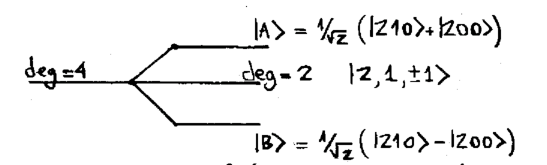
\includegraphics[width=0.6\textwidth]{images/teo2_20.pdf}
	\end{center}
	\caption{}
\end{figure} 

\subsection{Corrimiento de la energía a orden 2 (con degeneración)}

Sea que a orden uno se rompe toda la degeneración 
\[
	+ - = 0
\]
Entonces la corrección a segundo orden de la energía será:
\[
	+ - = E
\]
pues $\Braket{0_N^j|0_N^j}= 0$ pero 
\[
	=
\]
\[
	=
\]
falta desarrollo ...

\[
	E =
\]
donde $N$ es un estado degenerado.

\section{Estructura fina del átomo de hidrógeno}

La solución tradicional del átomo de H usa el potencial coulombiano. Esto desemboca en las funciones 
$\Ket{n,\ell,m}$, sin embargo la introducción de ajuste como {\it perturbaciones} rompe algo la degeneración.
\[
	cuentitas
\]
donde $a_0$ es el radio de Bohr, $\alpha$ es la constante de estructura fina .
Tenemos 
a) Corrección cinemática (relativista)
\[	
	0
\]
y esta corrección va como $W_{mv}/H_0 \sim \alpha^2$.

b) Acoplamiento spín-órbita
Se puede pensar considerando un $e^-$ en reposo con un protón orbitando que genera un $\vb{B}_{eff}$
\[
	W_{so} =
\]
y la corrección va como $W_{mv}/H_0 \approx \alpha^2$.

c) Término de Darwin o de contacto
\[
	=
\]
que va como  $W_{D}/H_0 \approx \alpha^2$.

Hay otras correcciones hiperfinas que provienen del spín del electrón y del spín del protón. Pero van como 
$\alpha^2/2000$.
Si consideramos el sistema con 
\[
	n=2
\]
serán ocho estados.
\[
	W
\]
y W es par ante $\Pi$ y sólo habrá elementos de matriz $\neq 0$ que sean de la misma paridad.
\[
	matriz
\]
y entonces $\Ket{2s}, \Ket{2p}$ no están conectados.

De manera que hay ocho estados $\Ket{n=2,\ell,m_\ell,s,m_s}$ que al calcular esta perturbación W resultan 
\begin{figure}[htb]
	\begin{center}
	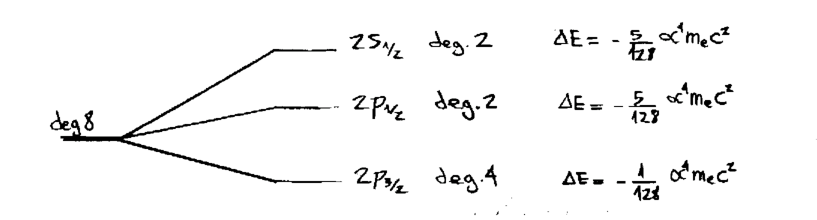
\includegraphics[width=0.9\textwidth]{images/teo2_21.pdf}
	\end{center}
	\caption{}
\end{figure} 
\[
	dg
\]
El cálculo para las correcciones hiperfinas no condice la experiencia. Se necesita aquí mecánica cuántica 
relativista. Los dos primeros niveles tienen la misma $\Delta E$ porque en MCR se ve que 
\[
	E = 
\]
es decir que no depende directamente de $\ell,s$.

Un sketch de los métodos perturbativos
\[
	H_0 = 
\]



% \bibliographystyle{CBFT-apa-good}	% (uses file "apa-good.bst")
% \bibliography{CBFT.Referencias} % La base de datos bibliográfica

\end{document}
